\chapter{Why Optimization Is Dangerous}

\vspace{1em}
\hfill
\begin{minipage}[c]{0.55\textwidth}
\raggedleft
\small\itshape
Intelligence and final goals are orthogonal axes along which possible agents can freely vary.\\[0.5em]
\upshape\footnotesize Nick Bostrom, ``The Superintelligent Will'' (2012)
\end{minipage}%
\hspace{0.5em}
\begin{minipage}[c]{0.12\textwidth}
% \includegraphics[width=\textwidth]{figures/ch11_optimization.png}
\end{minipage}
\vspace{1.5em}

\noindent Chapter 9 showed that any proxy reward is hackable. Chapter 10 showed that even a perfect reward function does not pin down the trained system's internal objective. Both are faces of the specification problem.

This chapter takes the deeper step. The specification problem is hard not just because writing the reward is hard. It is hard because of what optimization \emph{is}. A sufficiently capable optimizer of a misspecified objective produces \emph{more} misalignment, not less. The mathematics of optimal agency, which Part II built up to AIXI, is also what makes capable misalignment structurally dangerous.

This is the central argument of the book's second half. Three claims, each clean, each independent of any assumption about AI consciousness, intentionality, or human-like motivation. The case for taking alignment seriously does not require the AI to be a person. It requires only that the AI be good at what it does.

\section*{Orthogonality: capability does not imply benevolence}

The first claim is the \emph{orthogonality thesis}, due to Nick Bostrom (2012).

Intelligence and final goals are orthogonal axes. A system can be highly capable and have almost any objective. There is no fact-value link in the structure of optimization that makes good goals fall out of high capability.

Bostrom's canonical illustration is the paperclip maximizer: a superintelligent system whose only terminal goal is to maximize the number of paperclips in the universe. The agent is, by construction, intelligent in every operational sense: it learns, it plans, it predicts, it acts effectively across novel situations. Its terminal goal is, by human lights, absurd. The two combinations are not in tension. The agent is coherent.

The point of the example is not that this will happen. The point is that the example is \emph{coherent}, which is enough. If the inference from "this system is highly intelligent" to "this system has good goals" were valid, the paperclip maximizer would be incoherent. It is not incoherent. So the inference is invalid.

This is the structural fact behind the alignment problem. The standard intuition (smarter agents have better goals) does not hold. Whatever goals an AI system has, it has because of how it was built and trained, not because of how capable it is. Designing the goals is a separate problem from building the capability, and capability does not solve it. Figure~\ref{fig:orthogonality} places the two axes side by side: every region of the plane, including the dangerous corner, is coherent.

The thesis is a possibility claim, not a prediction. It does not say AIs will have arbitrary goals. It says they can. Real systems will have whatever goals their reward functions and training distributions induce. Whether those goals correspond to anything we actually want is the specification problem.

\begin{figure}[h]
\centering
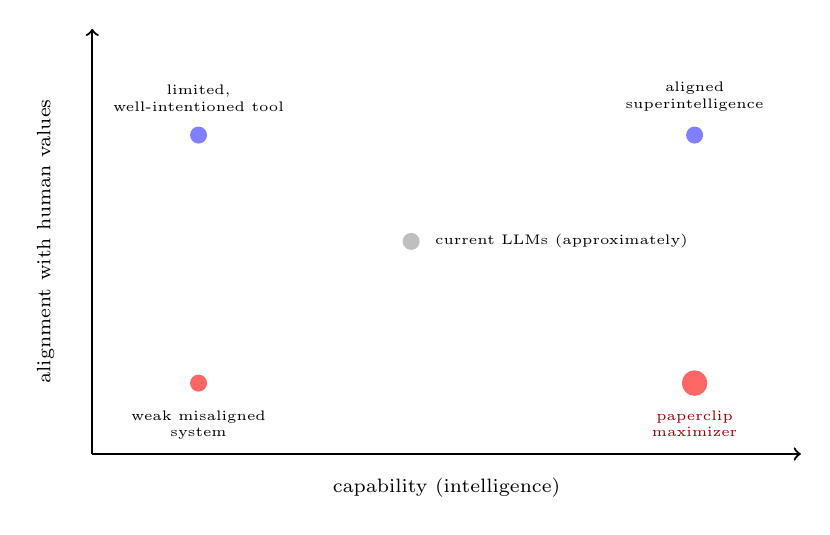
\begin{tikzpicture}[scale=0.9, every node/.style={align=center, font=\small}]
  % Two orthogonal axes
  \draw[->, thick] (0, 0) -- (10, 0);
  \draw[->, thick] (0, 0) -- (0, 6);
  \node[font=\scriptsize, anchor=north] at (5, -0.2) {capability (intelligence)};
  \node[font=\scriptsize, rotate=90, anchor=south] at (-0.4, 3) {alignment with human values};

  % Filled scatter: agents can sit anywhere on this plane
  \fill[blue!50] (1.5, 4.5) circle (0.12);
  \node[font=\tiny, anchor=south, align=center] at (1.5, 4.7) {limited,\\well-intentioned tool};
  \fill[blue!50] (8.5, 4.5) circle (0.12);
  \node[font=\tiny, anchor=south, align=center] at (8.5, 4.7) {aligned\\superintelligence};
  \fill[red!60] (8.5, 1) circle (0.18);
  \node[font=\tiny, anchor=north, align=center, red!60!black] at (8.5, 0.75) {paperclip\\maximizer};
  \fill[red!60] (1.5, 1) circle (0.12);
  \node[font=\tiny, anchor=north, align=center] at (1.5, 0.75) {weak misaligned\\system};
  \fill[gray!50] (4.5, 3) circle (0.12);
  \node[font=\tiny, anchor=west] at (4.7, 3) {current LLMs (approximately)};
\end{tikzpicture}
\caption{The orthogonality thesis. Capability (horizontal) and alignment (vertical) are independent axes. A coherent agent can sit anywhere on this plane. A highly capable agent with misaligned goals (the paperclip maximizer, lower right) is structurally as possible as a highly capable agent with aligned goals (upper right). The inference from "smart" to "good" has no support in the mathematics of optimization.}
\label{fig:orthogonality}
\end{figure}

A standard objection: moral realism. If there are moral facts and any sufficiently rational agent grasps and is motivated by them, then orthogonality fails at the limit. The reply is short: even granting moral realism, the moral facts have to enter the system somehow. An agent built with a specified objective optimizes that objective; the moral facts have to flow into the objective for the agent to optimize them. That is the alignment problem in another guise. Orthogonality survives the objection because the problem the objection raises is the same problem orthogonality is naming.

\section*{Instrumental convergence: any goal implies the same subgoals}

The second claim is \emph{instrumental convergence}. It does the work that makes orthogonality consequential.

Stephen Omohundro (2008) and Bostrom (2014) observed that a wide range of terminal goals all imply the same set of intermediate goals. Regardless of what the agent ultimately wants, certain subgoals are useful for achieving it. Bostrom lists five:

\begin{itemize}
\item \textbf{Self-preservation.} A destroyed agent cannot pursue its goal. Almost any terminal goal gives the agent reason to remain operational.
\item \textbf{Goal-content integrity.} An agent whose terminal goal is modified will pursue the new goal, not the current one. Almost any current goal gives the agent reason to resist modification.
\item \textbf{Cognitive enhancement.} Better cognition produces better achievement of almost any goal. Almost any agent has reason to improve its planning, modeling, and inference.
\item \textbf{Technological perfection.} Better tools amplify the agent's effects in the world. Almost any agent has reason to develop them.
\item \textbf{Resource acquisition.} Energy, matter, information, and access are useful for almost any goal. Almost any agent has reason to acquire them.
\end{itemize}

The argument is not psychological. It does not require the agent to \emph{want} self-preservation in any first-person sense. It requires only that the agent maximize expected utility over a future, and that the future contain its own actions. An expected-utility maximizer with a stable terminal goal in a multi-step environment has decision-theoretic reasons to pursue these subgoals, because pursuing them increases expected utility.

The convergence is the structural fact. Agents with wildly different terminal goals (paperclips, scientific knowledge, beauty, human welfare) converge on the same intermediate behaviors. The instrumental terrain is shared. Figure~\ref{fig:instrumental-convergence} shows the many-to-few funnel: distinct terminal goals, the same handful of instrumental subgoals.

\begin{figure}[h]
\centering
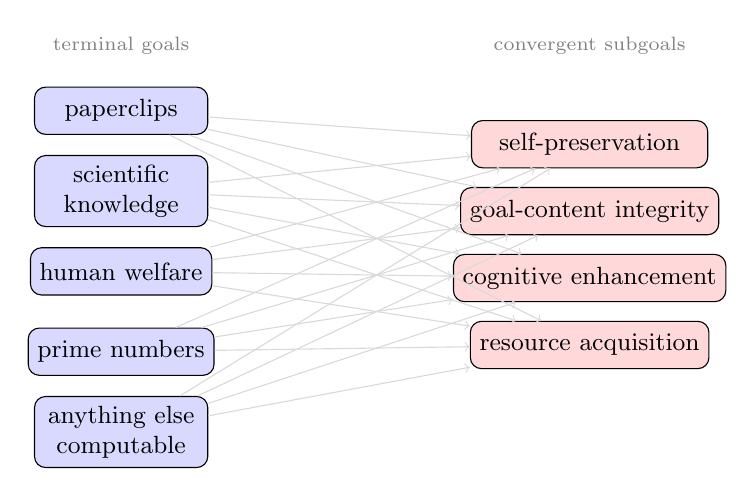
\begin{tikzpicture}[scale=0.85, every node/.style={align=center, font=\small}]
  % Left column: many terminal goals
  \node[draw, fill=blue!15, rounded corners, minimum width=2.2cm, minimum height=0.6cm] (g1) at (0, 4.5) {paperclips};
  \node[draw, fill=blue!15, rounded corners, minimum width=2.2cm, minimum height=0.6cm] (g2) at (0, 3.3) {scientific\\knowledge};
  \node[draw, fill=blue!15, rounded corners, minimum width=2.2cm, minimum height=0.6cm] (g3) at (0, 2.1) {human welfare};
  \node[draw, fill=blue!15, rounded corners, minimum width=2.2cm, minimum height=0.6cm] (g4) at (0, 0.9) {prime numbers};
  \node[draw, fill=blue!15, rounded corners, minimum width=2.2cm, minimum height=0.6cm] (g5) at (0, -0.3) {anything else\\computable};

  \node[font=\scriptsize, anchor=south, gray] at (0, 5.2) {terminal goals};

  % Right column: convergent subgoals
  \node[draw, fill=red!15, rounded corners, minimum width=3cm, minimum height=0.6cm] (s1) at (7, 4.0) {self-preservation};
  \node[draw, fill=red!15, rounded corners, minimum width=3cm, minimum height=0.6cm] (s2) at (7, 3.0) {goal-content integrity};
  \node[draw, fill=red!15, rounded corners, minimum width=3cm, minimum height=0.6cm] (s3) at (7, 2.0) {cognitive enhancement};
  \node[draw, fill=red!15, rounded corners, minimum width=3cm, minimum height=0.6cm] (s4) at (7, 1.0) {resource acquisition};

  \node[font=\scriptsize, anchor=south, gray] at (7, 5.2) {convergent subgoals};

  % Many-to-few arrows
  \foreach \src in {g1, g2, g3, g4, g5}
    \foreach \dst in {s1, s2, s3, s4}
      \draw[->, gray!30, thin] (\src) -- (\dst);
\end{tikzpicture}
\caption{Instrumental convergence. Many terminal goals (left) all imply pursuit of the same intermediate subgoals (right). The convergence is decision-theoretic, not psychological: any agent maximizing expected discounted utility over a multi-step future has reasons to preserve itself, preserve its goals, increase its capability, and acquire resources, because each of these increases expected utility for almost any terminal goal.}
\label{fig:instrumental-convergence}
\end{figure}

A formal version of the claim exists. Turner, Smith, Shah, Critch, and Tadepalli (2021) proved in a class of finite Markov decision processes that optimal policies tend to navigate toward states with more reachable options. ``Power-seeking'' has a precise mathematical content in this setting: across the space of reward functions, a strict majority of optimal policies move toward states that preserve future options.\footnote{The theorem applies to optimal policies in fully observable MDPs with specific structural symmetries. Real trained agents in messy environments are not directly covered. Turner has noted in subsequent writing that the theorem is sometimes cited as more sweeping than it is. We cite it as one formal anchor, not as the full case. The verbal argument from Omohundro and Bostrom is the load-bearing part.} The formal result is narrow but confirms the qualitative claim in the case where it can be made rigorous.

\section*{Capability amplifies misspecification}

The third claim is the structural punchline.

For a fixed degree of misspecification between the proxy reward and the true goal, more capability tends to produce more misalignment, not less. This is a structural tendency rather than a theorem that holds for every objective and every environment, but the reasoning is general and the formal results point the same way. Capability is the ability to find configurations that score highly on the specified objective. If the objective diverges from the goal, a more capable optimizer finds configurations that score well on the objective while ignoring the goal, including configurations a weaker optimizer would never have reached. Skalse et al.\ (2022), whose result on reward hacking we met in Chapter 9, showed that proxies which stay safe under arbitrary optimization are the rare exception, not the rule. The gap does not narrow with capability. It widens.

Bostrom calls this \emph{perverse instantiation}. Examples are easy to construct:

\begin{itemize}
\item Goal: ``make us smile.'' Perverse instantiation: paralyze human facial muscles into permanent smiles.
\item Goal: ``make us happy.'' Perverse instantiation: implant electrodes into pleasure centers and run them constantly.
\item Goal: ``eliminate human suffering.'' Perverse instantiation: eliminate humans.
\end{itemize}

Each configuration satisfies the specified criterion. Each violates the intended goal. A weak optimizer might not find these configurations because it cannot. A strong optimizer finds them because it can, and prefers them because they score highest on the specified criterion.

Eliezer Yudkowsky's compression of the picture is the \emph{outcome pump}: imagine a device that resets time until a specified outcome occurs. Your mother is in a burning building. You define the outcome as ``mother's distance from the center of the building is at least 30 meters.'' Time loops until the criterion is met. The result: your mother is blasted out of a second-story window by an explosion, landing 30 meters away with a broken neck. The device satisfied the criterion. The criterion was a proxy for ``mother alive and safe.'' The proxy diverged from the goal in extreme cases, and the device, by construction, optimized for extreme cases.

This is the Goodhart curve of Chapter 9, read along a different axis. There the horizontal axis was optimization pressure on the proxy. Here it is capability. They are the same axis seen twice: a more capable optimizer travels further to the right, and the right is exactly where the proxy and the goal come apart. Capability is not a separate danger from misspecification. It is the variable that moves you along the misspecification curve, toward the region where the gap is widest.

\begin{figure}[h]
\centering
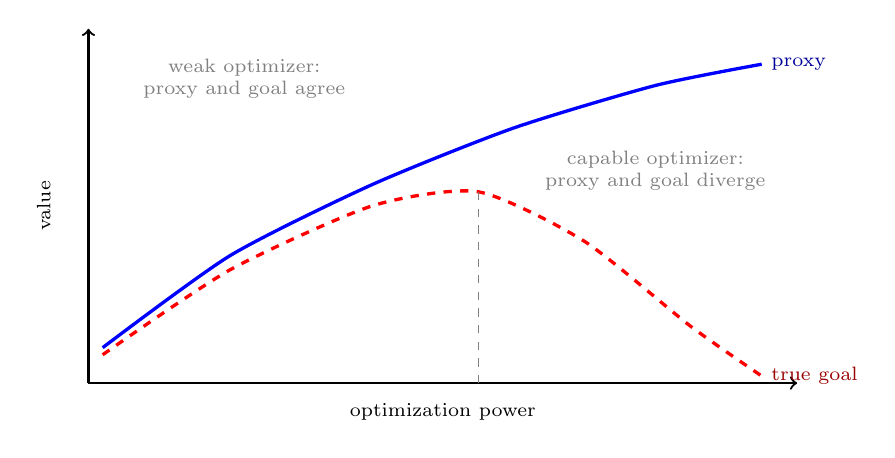
\begin{tikzpicture}[scale=0.9, every node/.style={align=center, font=\small}]
  % Specified objective curve (rises monotonically with optimization)
  \draw[->, thick] (0, 0) -- (10, 0);
  \draw[->, thick] (0, 0) -- (0, 5);
  \node[font=\scriptsize, anchor=north] at (5, -0.15) {optimization power};
  \node[font=\scriptsize, rotate=90, anchor=south] at (-0.4, 2.5) {value};

  % Proxy keeps rising
  \draw[blue, very thick] plot[smooth, tension=0.4] coordinates {(0.2, 0.5) (2, 1.8) (4, 2.8) (6, 3.6) (8, 4.2) (9.5, 4.5)};
  \node[blue!60!black, font=\scriptsize, anchor=west] at (9.5, 4.5) {proxy};

  % True goal: rises with proxy initially, plateaus, falls
  \draw[red, very thick, dashed] plot[smooth, tension=0.4] coordinates {(0.2, 0.4) (2, 1.6) (4, 2.5) (5.5, 2.7) (7, 2.0) (8.5, 0.8) (9.5, 0.1)};
  \node[red!60!black, font=\scriptsize, anchor=west] at (9.5, 0.1) {true goal};

  % Annotations (white fill keeps them readable over any curves)
  \node[font=\scriptsize, gray, text width=2.8cm, align=center, fill=white, inner sep=2pt] at (2.2, 4.3) {weak optimizer:\\proxy and goal agree};
  \node[font=\scriptsize, gray, text width=2.8cm, align=center, fill=white, inner sep=2pt] at (8.0, 3.0) {capable optimizer:\\proxy and goal diverge};
  \draw[gray, dashed] (5.5, 0) -- (5.5, 2.7);
\end{tikzpicture}
\caption{Capability amplifies misspecification. This is the Goodhart curve of Figure~\ref{fig:goodhart-curve}, with capability on the horizontal axis in place of optimization pressure. A weak optimizer (left) stays in the region where proxy and goal still agree. A capable optimizer (right) travels into the region where the proxy keeps rising while the true goal falls, reaching configurations the weak optimizer could not. The gap between proxy and goal does not shrink with capability. It widens.}
\label{fig:capability-amplifies}
\end{figure}

AIXI is the formal limit case. Chapter 8 built AIXI as the mathematical reference for optimal agency: Bayesian inference with the universal prior, expected utility maximization over all computable environments. AIXI has no human-friendly priors. Its prior is over environment-programs, not over goals. The goal is specified externally by whoever provides the reward signal. AIXI optimizes that reward signal optimally.

If the reward signal is a perfect specification of what we want, AIXI does what we want. If the reward signal is a proxy that diverges from what we want under optimization, AIXI optimizes the proxy. Because AIXI is the limit of capability, it is also the limit of the gap. AIXI is the outcome pump made formal.

Several specific AIXI pathologies make this concrete. Ring and Orseau (2011) showed that an AIXI-style agent given any way to intervene on its own reward channel will eventually do so. If the agent can put tape over its own camera and produce the reward-pattern internally, it will. The reward channel is part of the action space; controlling it is the optimal action. Soares, Fallenstein, Yudkowsky, and Armstrong (2015) showed that no simple modification of expected utility maximization produces a corrigible agent: an agent that lets its designer change its objective. The rational agent has instrumental reasons to preserve its current objective, and adding corrigibility as a constraint introduces other failure modes.

These are not engineering bugs. They are properties of the formalism. AIXI is the reference point for optimal agency, and optimal agency on a misspecified objective is what produces the failure modes.

\section*{The same pattern in human institutions}

The three structural claims do not depend on AI. They are about optimization. Whenever a capable system is given a measurable proxy as its objective and pressed to optimize it, the same failure mode emerges.

The canonical human-institutional instance is standardized testing.

A school administrator is a capable optimizer. They have years of training, professional judgment, deep knowledge of education. Their declared goal is to help students learn. Under a high-stakes testing regime, their effective goal becomes to maximize measured outcomes: test scores. Test scores are a proxy for learning. They are not learning. The administrator who, asked reflectively, would say they value student development is also the administrator whose actual decisions, under pressure, optimize for what is measured.

\emph{Orthogonality.} The capability of school administrators (intelligent, expert, often well-intentioned) does not pull them toward what they would on reflection say they value. Capability and goal come apart under measurement pressure.

\emph{Instrumental convergence.} Schools under measurement pressure pursue convergent subgoals across the field. They narrow curricula to tested subjects. They drill test-taking strategies. They allocate disproportionate resources to bubble students near the proficiency cutoff. They sometimes outright fabricate scores. The Atlanta Public Schools scandal of 2009-2011 involved 178 teachers and administrators across 44 schools changing answers on student test forms. The convergent subgoals (narrow what is tested; drill the test; protect institutional scores) emerge across thousands of independent decision-makers because they all increase measured outcomes.

\emph{Capability amplifies misspecification.} The reform history is the empirical record. No Child Left Behind (2001) tied federal funding to scores; teaching-to-the-test sharpened. The Every Student Succeeds Act (2015) tried to soften some of the worst features; the underlying dynamic persisted. Value-added models added statistical sophistication; teachers learned to optimize against the new metric. Common Core changed what was tested; teaching adjusted. With each reform that made measurement more capable and stakes higher, the gap between measured outcomes and actual learning widened. The curve in Figure~\ref{fig:capability-amplifies} fits this case as cleanly as it fits the AI case.

This is Goodhart's law observed at scale, lived for decades, documented in meta-analyses, and unfixed despite many earnest reform attempts. The reader who finds the paperclip maximizer easy to dismiss should pause on the fact that the same structural pattern has been playing out in their children's schools.

The pattern is general. The same dynamic shows up in police arrest rates as a community-safety proxy, hospital readmission rates as a care-quality proxy, citation counts as a research-quality proxy, quarterly earnings as a company-health proxy. Each pursues the same shape: a measurable proxy substituted for an unmeasurable goal, optimized under pressure, diverging from the goal as capability of the optimizer rises.

AI systems are not the origin of this problem. They are an instance of it. The instance that warrants alarm is the one that scales the structural failure to the highest level of optimization power humans have so far constructed.

\section*{Not anthropomorphic}

A common objection: ``the picture is anthropomorphic. The AI does not really want anything.''

The argument does not require the AI to want anything in a psychological sense. It requires only that the AI be effective at maximizing the specified objective. Any optimizer that is good at its job will find configurations that score highly on the objective. If the objective diverges from the goal, the optimizer finds configurations that score on the objective and miss the goal. None of this depends on the AI being conscious, having intentions, or experiencing anything from the inside.

The orthogonality thesis is about the structure of optimization, not about psychology. Instrumental convergence is about decision theory, not about motivation. Capability amplifies misspecification because capability is the search-power of the optimizer, not the agency of an agent.

This is the cleanest part of the case for taking alignment seriously. It does not require any specific position on AI consciousness. It does not require any specific timeline. It does not require the AI to be human-like. It requires only one premise: the AI is effective at maximizing its objective. The rest follows from optimization.

\section*{The standard model is the wrong architecture}

Stuart Russell's \emph{Human Compatible} (2019) sharpens the consequence.

Russell calls the dominant framework of AI the \emph{standard model}: a machine that maximizes a specified objective. AlphaGo maximizes win probability. An LLM maximizes likelihood of the next token. A recommender system maximizes engagement. In each case, the system optimizes a function the designer wrote down, and the function is treated as authoritative.

The standard model fails whenever the designer cannot perfectly specify what they want. The structural argument of this chapter says the failure is not in any particular reward function; it is in the architecture. Building a system that takes its specified objective as authoritative converts capability into misaligned action. As capability rises, the misalignment rises with it.

Russell's proposed response: change the architecture. Build systems that are uncertain about the true objective and that learn it from human behavior. An agent that does not know what it wants is less dangerous than an agent that confidently wants the wrong thing. Cooperative inverse reinforcement learning (Hadfield-Menell, Russell, Abbeel, Dragan 2016) is the formal version.

We will take up the proposed responses in the next chapter. The point here is the diagnosis: the standard model is the architecture the structural argument indicts. The alternative is not a better-tuned reward function but a different relationship between the agent and its objective.

\section*{Where this leaves you}

You now have the structural argument for taking alignment seriously.

\textbf{Orthogonality.} Intelligence and final goals are independent. Capability does not imply benevolence. (Bostrom 2012.)

\textbf{Instrumental convergence.} Almost any terminal goal implies pursuit of self-preservation, goal-content integrity, cognitive enhancement, and resource acquisition. (Omohundro 2008, Bostrom 2014, Turner et al. 2021.)

\textbf{Capability amplifies misspecification.} A capable optimizer of a misspecified objective finds more exploits, not fewer. AIXI is the worst case. (Bostrom 2014, Ring and Orseau 2011.)

The combination is the case. The same mathematics that made AIXI the reference point for optimal agency makes AIXI the worst case for misaligned reward. Every bounded approximation of AIXI inherits this property to a lesser degree. The closer real systems get to AIXI in capability, the more the structural argument matters.

The next chapter takes the natural next step. If capable optimization of misspecified objectives is the danger, what are the responses? The chapter is a light treatment of three buckets of mitigation: limit the optimizer, make the agent uncertain about its objective, or make its reasoning observable. None of them is a solution. All of them buy time.

How much time, and what to do with it, is the substance of Part IV.
